
% Chapter 5

\chapter{Implementation} % Write in your own chapter title
\label{Chapter 5}
\lhead{Chapter 5. \emph{Implementation}} % Write in your own chapter title to set the page header

\section{Tools for implementation}
To develop this proposed system, we use some tools to implement this system which is given below:
\begin{itemize}
\item Android 3.5 or above with java
\item Php MySQL
\item Php Storm
\item Postman
\item MATLAB
\item Python IDE (Spyder, Anaconda)
\end{itemize}


\subsection{Android 3.5 or above with java}
We used an Android studio to develop the android applications. Actually, we have been made three applications on android that is admin app, user app and data capturing app. We used java language to make these applications.

\subsection{Php MySQL}
We use Php MySQL to make the database of our application. It is necessary for our system to make the database because the information of the rooms which the user can see, fetch from database. We deployed the database on the server. So that, when the user connects with the application, information of the room fetch from the server.

\subsection{Php Storm}
We use Php storm for making the scripts in the database. Actually, the android studio could not connect to the Php MySQL database directly. To connect the android studio with Php MySQL, we had to make the scripts of database in Php storm. This tool helps us to connect the database with android studio.

\subsection{Postman}
After creating the scripts of database in php storm, we use this software for testing. For Example, when we make the database connection file in php. We check that this file connect to database or not. In this way, we check one by one all php files either these are working or not.

\subsection{MATLAB}
For the compilation of BLE beacons dataset, we use MATLAB. Actually, the dataset of our department is being captured on different devices, the number of files is generated by data capturing app. To compile all over the files, we use this tool to make our work linier.

\subsection{Python IDE}
We use Python IDE such as Anaconda and Spyder to train the model of machine learning. Actually, we use different libraries of python such as tensor flow, numpy, matplotlib.py, pandas and preprocessing from sklearn. To train the model, these libraries are necessary to import. By using these libraries, we applied different algorithm such as k-NN, ANN and Random Forest (RF) to train the model.
\clearpage

\section{Implementation of Machine Learning Algorithms}

We focused to train our ML model to high precsion because this project aims to predict the indoor location of the user's mobile device. As, we are not predicting the outdoor location on the map, we need to more focus on the signal strength of the devices and the accuracy of our train models. To analyze our dataset, we didn't rely on any one classifier. Three algorithms are used for the purpose of training the model which includes knn, ann and random forest. These three were being decided by analyzing their predicting methods. knn works on the neighbourhood classification, random forest works after making multiple random decision trees by making subsections of the dataset while ann works on neural networks by making hidden layers. We choose three algorithms because after analying their comparison, we choose the best one whose accuracy and precision is high. The detailed implementation and description of these algorithms is described below.

\subsection{k- Nearest Neighbours}

k-NN is the simplest and supervised machine learning algorithm. Here we used it for multi-classification. k-NN uses data and classify new data points based on majority vote of the nearby points. Before the implementation of k-NN, we have to tell the values of the hyper parameters of k-NN. The basic parameters for k-NN algorithm are:

\textbf{Number of nearest neighbors}

We have to choose number of nearest neighbors in order to find the class of new data point based on the majority votes from these nearest neighbors.

\textbf{Distance measure}

There are two major distance measure Euclidean and Manhattan. We have to choose one of them as a distance measure criterion. Figure 6 shows the Euclidean distance measure and Figure 7 shows Manhattan distance measure.


\textbf{Weights assigned to neighbors}

The weight parameter has two choices: ‘distance’ and ‘uniform’. The ‘uniform’ weight means that each of the k neighbors has equal vote, whatever its distance from target point. The ‘distance’ measure means that in the k neighbors, the neighbor who is close to target point has given more weight than the neighbor who is far from the target point.

This figure represents impact of choosing the weight assigning criterion on accuracy score.
\begin{figure}[h]
  		\centering
    		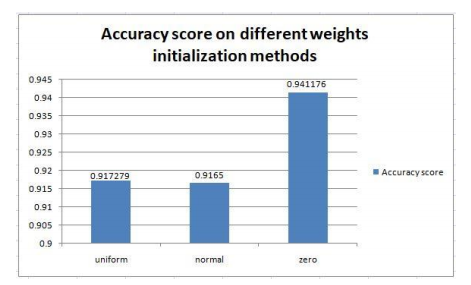
\includegraphics[scale=0.85]{./Figures/weights}
\caption{Impact of choosing the weight assigning criterion on accuracy score.}
\label{fig:1}
 		\end{figure}


\subsubsection{Hyper-parameters tuning:}

Before we implement k-NN, we need to find the best values for parameters at which accuracy is maximum. For this purpose, we use GridsearchCV function to test for all possible combinations of n neighbors, weights, distance in order to find out best parameters at which accuracy is maximum. We take values of k neighbors from 1 to 26, weights = {uniform, distance} and distance measure = {‘euclidean, manhattan}, then we try to find the best possible combination. Figure 25 represents the impact of choosing the distance measure on accuracy score.
\begin{figure}[h]
  		\centering
    		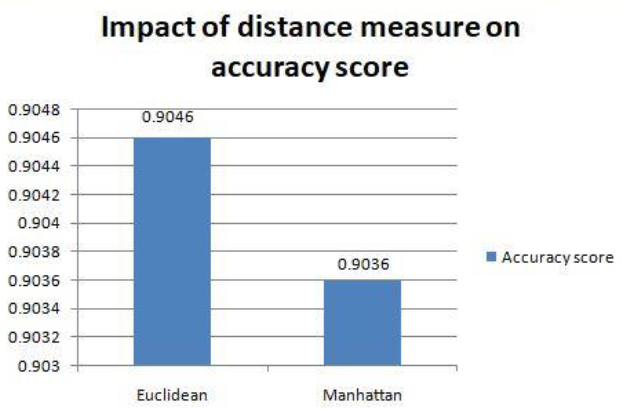
\includegraphics[scale=0.65]{./Figures/distance}
\caption{Impact of choosing the distance measure on accuracy score.}
\label{fig:2}
 		\end{figure}

This graph represents the impact of choosing the number of neighbors on accuracy score.
\begin{figure}[h]
  		\centering
    		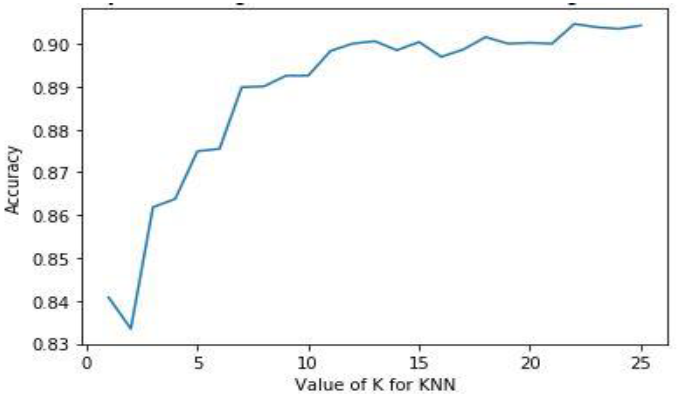
\includegraphics[scale=0.65]{./Figures/neighbours}
\caption{Impact of choosing the number of neighbors on accuracy score}
\label{fig:3}
 		\end{figure}

Hence, after checking the impact of choosing different values of parameters on accuracy score, we find out that best parameters are:
\\
Distance measure: 'euclidean'\\
Number of neighbors: 22\\
Weights: 'uniform'\\


\subsubsection{Methodology for data training}

1-Input: Data set and best parameters for k-NN.\\
2- Split the data into training set (75 percent) and testing set (25 percent). We use ‘startify’ so that the train and test sets have approximately the same percentage of samples of each target class as the complete set.\\
3- Built the k-NN classifier by feeding it with the training data and best parameters.\\
4- Train the model and store the model on the disk.\\
5- Plotting of confusion matrix.\\
6- Calculate accuracy, precision and recall for training and testing data.\\



\subsection{Random Forest Classifier}
Random forest is one of the most powerful supervised machine learning algorithms. It is capable of performing both classification and regression but here we use this algorithm for multi-classification. For this purpose, it creates multiple decision trees in the form of forest by selecting random samples from dataset for each decision tree. 

\textbf{Why we are using random forest? }

The over fitting problem will never come when we use the random forest algorithm in any classification problem. The random forest algorithm can be used to identify the most important features out of the available features from the training dataset. It means we don’t have need to normalize the features. Tree models can handle both continuous and categorical data and can model nonlinear relationships

\subsubsection{Description of Hyper-Parameters:}

To train model on different hyper-parameters, it is necessary to pick out best parameters on which accuracy becomes high. Some parameters are: n estimators are the number of trees in the forest. Higher the number of trees, higher is the prediction accuracy. max features is maximum number of features considered for the best split. max node is the  maximum number of nodes in which dataset can split. Batch size  indicates the number of samples per batch.random state defines random selection to compare between different models.
Except these values, we also trained our model on different values of hyper parameters and plot their accuracy response in the form of graphs as shown below:

\begin{figure}[h]
\begin{center}
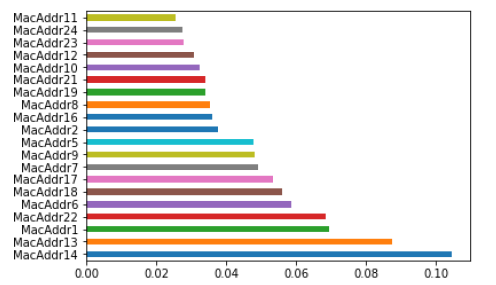
\includegraphics[scale=0.85]{rffeature}
\caption{Feature Importance Graph}
\label{fig:4}
\end{center}
\end{figure}

\clearpage

\begin{figure}[h]
  		\centering
    		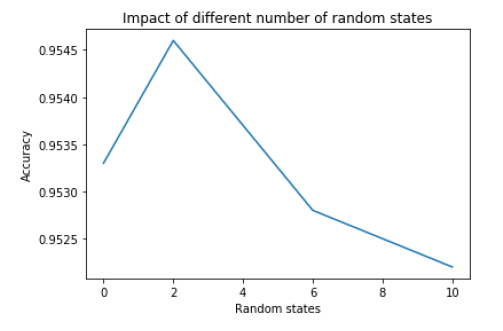
\includegraphics[scale=0.8]{./Figures/rfrs}
\caption{Impact of different number of random states}
\label{fig:5}
 		\end{figure}

\begin{figure}[h]
  		\centering
    		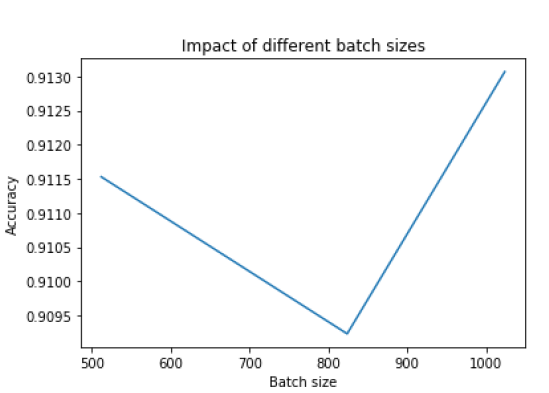
\includegraphics[scale=0.7]{./Figures/rfbs}
\caption{Impact of different number of batch sizes}
\label{fig:6}
 		\end{figure}

Hence, after checking the impact of choosing different values of parameters on accuracy score, we find out that best parameters are:
n estimators: 10\\
max features: 24(all)\\
max node: 1000\\
Batch size: 1024\\
random state: 1\\

\subsubsection{Methodology for data training}
1. Present a dataset containing number of training samples characterized by multiple features and target feature.\\
2. Random forest selects ‘m’ features from the total features randomly.\\
3. Select the root node using best split and split these nodes into daughter nodes\\. 
4. Repeat above steps to form various decision trees until maximum number of nodes reached.\\
5. Create leaf nodes which are further used to predict new query instances. \\
6. Make and initialize a tensorflow session to train the model. \\
7. Calculate accuracy of training and testing model. \\
8. Predict the outcome using these decision trees.\\
9. Measure the outcome or target label predicted by each tree.The target with the highest vote is considered as the final prediction of the random forest algorithm. 


\subsection{ANN}
ANN is a powerful deep learning algorithm inspired by biological structure of neurons. Information flows in the hierarchical form. We have used 2-layered neural network for our multi-classification problem because in many internet sources, we find out that 2-layered network is sufficient. The input layer consists of input neurons. Those neurons transmit data to
the next layer, which in turn sends the output neurons to the output layer. Figure 30 shows the structure of Neural Network.

\begin{figure}[h]
  		\centering
    		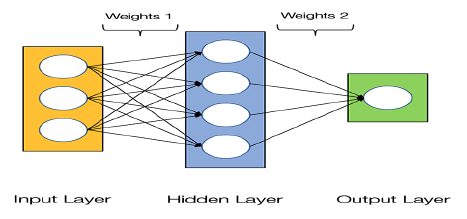
\includegraphics[scale=0.85]{./Figures/ANN}
\caption{Structure of neural network}
\label{fig:7}
 		\end{figure}

The basic parameters for ANN algorithm are:
1- Batch size and Epochs:\\
Batch size tells that how many samples are used to calculate the error. Number of epochs controls the number of complete passes through training dataset. One epoch is comprised of feed forward and back propagation. In feed forward, we calculate the predicted outputs and then calculate the error using any error measure formula. Then, in back propagation, this error is used to update the weights.\\
2- Optimization Algorithms:\\
There are many optimization algorithms like ‘SGD’, ‘Adam’, ‘Nadam’ etc. We can use any of the optimization algorithms and it is used for updating the weights.\\
3- Weight Initialization Methods:\\
There are many weight initialization methods like ‘zero’, ‘normal’, ‘uniform’. We can use any of the weight initialization methods and it is used for initializing the weight vector. ‘zero’ method initializes the weight vector with all zeros.\\
4- Activation Function:\\
Each neuron has an activation function that gets the input from previous layer which combines with associated weights and then passes to the activation function that produce output and then this output pass to the next layer.\\
5- Number of neurons:\\
Each layer has many number of neurons as you can see in the Figure.

\subsubsection{Hyper-parameters tuning:}

Before we implement ANN, we need to find the best values for parameters at which accuracy score is maximum. For this purpose, we use GridsearchCV function to test for all possible combinations. Here are the results:
This figure shows the impact of batch sizes on accuracy score.


\begin{figure}[h]
  		\centering
    		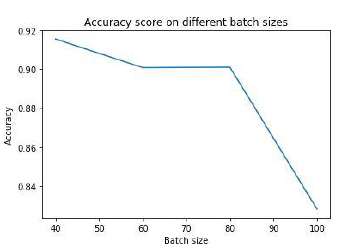
\includegraphics[scale=0.95]{./Figures/annbs}
\caption{Impact of batch sizes on accuracy score.
}
\label{fig:8}
 		\end{figure}
\clearpage
This figure shows the impact of epochs on accuracy score.

\begin{figure}[h]
  		\centering
    		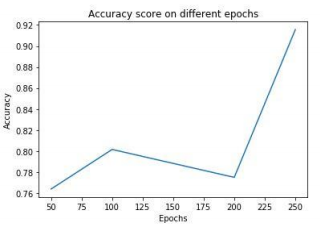
\includegraphics[scale=1.0]{./Figures/epochs}
\caption{Impact of epochs on accuracy score.}
\label{fig:9}
 		\end{figure}
This figure shows the impact of number of neurons on accuracy score.

\begin{figure}[h]
  		\centering
    		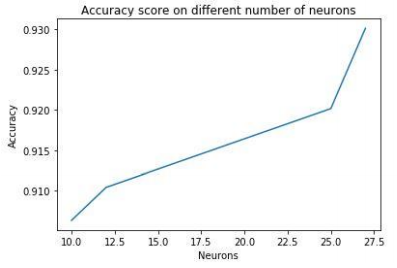
\includegraphics[scale=0.85]{./Figures/neurons}
\caption{Impact of number of neurons on accuracy score.}
\label{fig:10}
 		\end{figure}
\clearpage

This figure shows impact of weight initalization methods on accuracy score.
\begin{figure}[h]
  		\centering
    		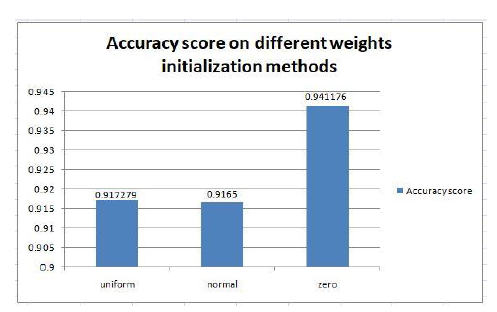
\includegraphics[scale=0.75]{./Figures/annmethods}
\caption{Impact of weight initalization methods on accuracy score.}
\label{fig:11}
 		\end{figure}


This figure shows the impact of different optimization algorithms.

\begin{figure}[h]
  		\centering
    		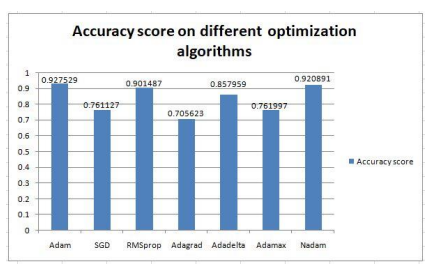
\includegraphics[scale=0.82]{./Figures/optalgos}
\caption{Impact of different optimization algorithms.}
\label{fig:12}
 		\end{figure}
\clearpage

We also tune activation functions { 'relu', 'tanh', 'sigmoid', ‘linear’}. All of them gave same accuracy score.
Hence, after checking the impact of choosing different values of parameters on accuracy score, we find out that best combination has following values:
Batch size: 40\\
Epochs: 250\\
Optimization Algorithm: ‘Adam’\\
Weight Initialization Methods: ‘uniform’\\
Activation Function: ‘relu’ for hidden layer and ‘sigmoid’ for output layer\\
Number of Neurons for hidden layer: 27\\

\subsubsection{Methodology for data training}

1- Input: Data set and best parameters for ANN.\\
2- Split the data into training set (75 percent ) and testing set (25 percent). We use ‘startify’ so that the train and test sets have approximately the same percentage of samples of each target class as the complete set.\\
3- We apply label encoder to the output vector that encode classes that are in string format into integers. Then we apply to categorical that convert a class vector into binary class matrix.\\
4- Built the 2-layered ANN classifier by feeding it with the training data and best parameters.\\
5- Train the model and store the model on the disk.\\
6- Plotting of confusion matrix.\\
7- Calculate accuracy, precision and recall for training and testing data.


\clearpage
\section{Implementation of Android applications}
Actually, our proposed system has three Android applications.
\begin{itemize}
\item Data Capturing App
\item Admin Android App
\item User Android App
\end{itemize}

\subsection{Data Capturing Application}
The functional requirements and the implementation of Data Capturing Application are as follows:
\subsubsection{User can enter his name or ID}
The user who is going to capture the fingerprints of RSSI values, he can enter his name or ID because after capturing the data, file saves with user’s name and time at which he generates file(format is shown in figure). Multiple users and multiple devices of user can capture data for a same project in same working hours. So, at a same time, multiple files can be generated in separate mobile devices. But, replacement issue occurs when we gather all of them, some files would remain and some would be deleted. So, to avoid this issue, we make a tab for user where he can enter his name or ID.
\subsubsection{Scanning of nearby BLE Bluetooth devices}
The scanning of nearby BLE Bluetooth devices starts when a user press a startscan button on the screen of the Android application. This functionality will search the nearby 4.0+ Bluetooth devices and show the signal strength which a mobile device is capturing from each nearby BLE device. Meanwhile, the scan stops after it shows fingerprints of all the nearby devices on the screen as shown in figure.
\subsubsection{Restart scan and capture RSSI fingerprints}
The Bluetooth scanning stops while it scans all the nearby devices, but there is a big problem that occurs. The user can immediately change his location while moving from one room to the other room or corridor or some other location in the room or department. At that time he is near another beacon after changing his location instead of which whose RSSI values he was capturing so there becomes a room label issue. He was not capturing the signal strength of that particular room whose label was assigned at the start. In order to capture the fingerprints of the updated location of the user we need to rescan its nearby devices so that application can capture nearby devices for that updated location.
\subsubsection{Generate csv file of captured data}
When the fingerprints of mobile device from each nearby beacons are captured and they can be seen on the screen. User press the “Generate file” button in order to save that data in the form of csv format file in his mobile phone storage. The number of files generated per press of the button depends on the number of iterations of scanning (according to delay factor) which we give to the process at the start
\subsubsection{Add delay function to slower the process}
Our application generates a single file after a full scan of nearby devices. Once scanning becomes stop, it will save the data in one csv file and then start the rescanning process. When we generate multiple files without delay factor, it miss some files because the process of file generation is slow than rescanning. In this case, the rescanning of nearby BLE devices starts after before the generation of new file so in order to not miss any file we add a delay factor. Delay factor will start generating the file after rescanning has been done.
\subsubsection{Allow user to generate files in iterations according to delay time}
User allows to generate multiple files by single press for efficiency. In less time and by less effort, he can generate files after some delay. We use a delay of 5 seconds, it means every file is being generated after 5 seconds and this is enough time to rescan the device.



\subsection{Admin Android Application}

\subsubsection{Design Database of Admin App}
It is the rule to develop the software is that create database for our system. So, we also make the database design first. We make 5 tables of database that is:
\begin{itemize}
\item Admin
\item Room 
\item Room Members
\item Office Hours
\item Pictures
\end{itemize}
Actually, in our system, Admin will do login and signup to handle the administration purpose. For this purpose, we made the Admin Table. Anyone can be the admin. So, we can get the data of admin when he/she register in our system. Admin table is used to save the record of Admin. Then, we make the table of Room Information. As you know that, the department of every University has rooms. To store the information of every room in the department, we made room information table. After this, we made the Room Members table. As you know, every department has the rooms. The room may be class room, lab and the office of the teacher. If the room is the office of the teacher, then we have to store the information of the teachers. We have to store the information such as teacher name, teacher qualification, teacher designation, teacher office hours. To store the information of the office hours of the room members, we made Office Hours table. This office hours tables have store the information of the starting time, ending time and week day of room member. At the end, we store the images of the room. Actually, we want that user easily access the room. For this purpose, we show images of the specific room in which user stands. To store the pictures of the room, we made Picture Info Table.   
Our Database design is as follows:
\begin{figure}[h]
  		\centering
    		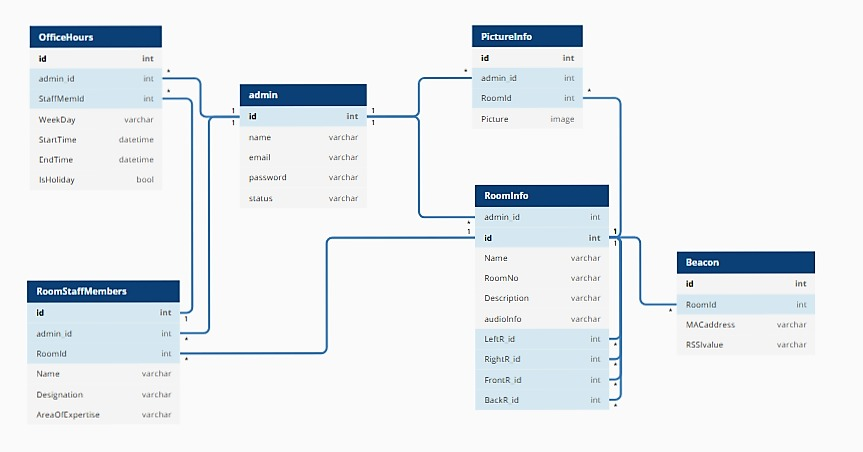
\includegraphics[scale=0.5]{./Figures/dbdesign}
\caption{Database design diagram}
\label{fig:13}
 		\end{figure}

\clearpage

\subsubsection{Creating Web services for our App}

After creating the database, we need to create web services for our project. Actually, the problem of our system is that it does not connect to the database directly. So, we need some medium between Admin App and server. For this purpose, we create web services. It is called API’s. It is also called RESTful API.
Now, we discuss about how to create web services. To create the web services, we use php only. We can do php code on any framework. But for our system, we do php coding on Php storm. The relationship between the database, server and android app is as follows: 
\begin{figure}[h]
  		\centering
    		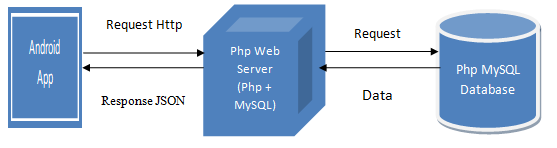
\includegraphics{./Figures/relation}
\caption{Relationship between database server and android application}
\label{fig:14}
 		\end{figure}

In this way, we connect our Admin App with php MySQL database. There are following steps to create the web services that are as follows:

\begin{itemize}
\item First of all, we create a php project. Remember that, we use Php storm for this purpose.
\item Then we make the database connection file. Our database filename is DbConnect.php. We used this file to create the database.
\item After this, we create the files for two operations, one is for Admin Signup and the other is for Admin Login. This file name is called API.php. We handle all the API calls in this file.
\item We also validate the parameters in the Api.php file. Validating parameters is important for users.
\item Because, we wanted to do CRUD operation for rooms. We make another file called RoomOperation.php. The main functions were created in this file. Some database queries are also written in this file. The function of AddRooms(),UpdateRooms() and deleteRooms() are also create in this file.
\item In RoomOperation.php, we did not only make the functions for room. We also created the functions of Room members We also created the functions of AddRoomMemberInfo(), UpdateRoomMemberInfo() and deleteRoomMemberInfo().
\item In RoomOperation.php, we did not only make the functions for room. We also created the functions of office hours of Room members. We also created the functions of AddOfficeHours(), UpdateOfficeHours () and deleteOfficeHours ().
\item After this, we make the file of RoomApi.php. This file handles all the API calls for database operations such as add, edit and delete.
\item At the end, we make UploadImgToServer.php file. Because, we wanted to upload rooms images on server. For this purpose, we created this file.
\item At the end, we had tested the all file using REST client. In this scenario, our REST client is POSTMAN. This software is used for testing purposes
\end{itemize}


By follow these steps, we create the web services for our android Application. Now, we move to the android part of our Admin App.
\subsubsection{Login and Signup of Admin App}
After creating the web services, we develop the Admin App on Android Studio.

\begin{itemize}

\item First of all, we create the xml file. The xml file in android studio is used to make the front end. So, it is necessary to use xml file for making the Front end of android app. We made the front end which is easy to use for user. Our front end is user friendly. We can use different layouts for frontend. But in our system, we used Relative layout.
\item Now, we move to backend coding. We make java classes for this purpose. Actually, we want to connect the android with database. For this purpose, we made the URLs.java file. We give the URL of php scripts in android app.
\clearpage
 The format of URL is as follows:
 
\begin{figure}[h]
  		\centering
    		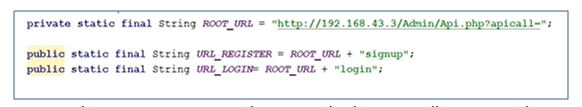
\includegraphics[scale=0.9]{./Figures/URL}
\caption{Format of URL of php scripts in Android application}
\label{fig:15}
 		\end{figure}

\item By using these URLs, we connect the app to database. Actually, we use online database. That’s why, there are some conditions to connect this app to database that is:

a)	Your mobile is connected to the internet\\
b)	The IP Address of Wi-Fi is same for server and your mobile phone.\\
c)	Your mobile is connected with the same internet which is connected to the server.
 
\item After connecting the database,   we do some backend code of java. We write the code which helps Admin to Login and Signup in this App. We created two java classes for this purpose. One was AdminLogin.java and other was AdminSignup.java.
\item After making the java file of Admin Login and Admin Signup, we tested it.
\end{itemize}


\subsubsection{Add/Edit/del Room information}
After login, Admin can add, edit and delete the room information. To do this, he/she follow these steps which are given below: 
\begin{itemize}

\item Admin show the list view in which the information of the room is present. To implement this activity, we use listview in this activity. We add textboxes in the listview in which the room number is shown.
\item If Admin click the add button, then it moves to Add Room activity. To implement this, we make the frontend using xml files of android. Then, we do backend code on Add button click event. This button helps us to add the information from the android app to database. 
\item After clicking the room which is on the listview, the dialogue box is shown. It asks the Admin that do you want to delete or edit. To implement this feature we dynamically create the dialogue box. For this purpose, we used libraries of android which support dialogue box. 
\item If Admin clicks the delete, then the room from the listview will delete. For this purpose, we get the Room Id which deletes the record of room from database table of Room. 
\item If Admin clicks the Update button, then another activity is open, in which all data of that room is present. Admin can update the room name, room number and so on. For this, we also get the room id and update the record of that room on the database. The update button helps us to connect to the database. So that, the values of that room is updated.
\item It is possible when Admin connect to this Application to the internet.
\end{itemize}

\subsubsection{Add/Edit/del Room Member information}
After this, Admin can add, edit and delete the room member information. To do this, he/she follow these steps which are given below: 
\begin{itemize}

\item Admin show the list view in which the information of the room member is present. To implement this activity, we use listview in this activity. We add textboxes in the listview in which the room member name is shown.
\item If Admin click the add button, then it moves to Add Room Member activity. To implement this, we make the frontend using xml files of android. Then, we do backend code on Add button click event. This button helps us to add the information from the android app to database table of Room Member Info. 
\item After clicking the room member name which is on the listview, the dialogue box is shown. It asks the Admin that do you want to delete or edit. To implement this feature we dynamically create the dialogue box. For this purpose, we used libraries of android which support dialogue box. 
\item If Admin clicks the delete, then the room member name will delete from the listview. For this purpose, we get the Room member Id which deletes the record of room member from database table of Room Member. 
\item If Admin clicks the Update button, then another activity is open, in which all data of that room member is present. Admin can update the room member name, room member qualification and so on. For this, we also get the room member id and update the record of that room member on the database. The update button helps us to connect to the database table of room member info. So that, the values of that room member is updated.
\item It is possible when Admin connect to this Application to the internet.

\end{itemize}

\subsubsection{Add/Edit/del Office Hours of Room Member}
 After this, Admin can add, edit and delete the Office Hours of Room Members. To do this,     he/she follow these steps which are given below: 
\begin{itemize}
\item Admin show the list view in which the information of the Office Hours of Room Members is present. To implement this activity, we use listview. We add textboxes in the listview in which the timings of room members is shown.
\item If Admin click the add button, then it moves to Add Office Hours activity. Admin can add the start time, end time, week days and so on To implement this, we make the frontend using xml files of android. Then, we do backend code on Add button click event. This button helps us to add the information from the android app to table of database that name is Office Hours. 
\item After clicking the timings of room members which is on the listview, the dialogue box is shown. It asks the Admin that do you want to delete or edit. To implement this feature we dynamically create the dialogue box. For this purpose, we used libraries of android which support dialogue box. 
\item If Admin clicks the delete, then the office timings of room members from the listview will delete. For this purpose, we get the Id of Office Hours. We get this id from the Admin clicks on the listview. The record of this id will delete from database table of Office Hours.
\item If Admin clicks the Update button, then another activity is open, in which all data of the office timings of room members is present. Admin can update the start time, end time, week days and so on. For this, we also get the id and update the record from the Office Hours table of database. The update button helps us to connect to the database. So that, the values of that table is updated.
\item It is possible when Admin connect to this Application to the internet
\end{itemize}


\subsubsection{Add Pictures of Room}
At the end of the implementation of Admin App, we add the functionality of Add pictures. For this purpose, we upload the image to the server. It is not easy to upload the image to the server. But we did it. Actually, images are not added directly to the database. So, we save the link of the image which is uploaded to the server in database. Actually, we made this feature for the ease of user. The user can see the room information in the form of pictures. The scenario to upload image to the server is shown below:

\begin{figure}[h]
  		\centering
    		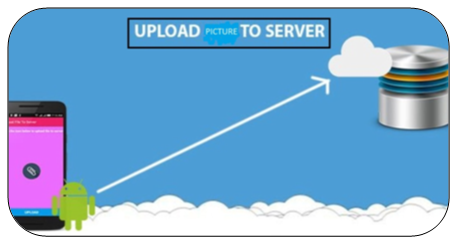
\includegraphics[scale=0.75]{./Figures/uploadimage}
\caption{Scenario to upload image to the server}
\label{fig:16}
 		\end{figure}


Due to shortage of time, we don’t implement the features of edit/delete. It is very difficult to edit and delete the images from the database indirectly. But in future, we try to add these functionalities. Admin can also edit and delete the pictures from the server.

\subsection{User Android Application}
Now, we describe some points of the implementation of user application which are as follows:

\subsubsection{Integrate trained ML model with user app.}
After training the model, we have to integrate this model with user app. For this purpose, we choose tensorflow lite. To execute the trained model with tensorflow lite. We have to convert model file to .tflite .Actually, tensorflow lite only considered .tflite file.
In an android application, we have to embedded the .tflite file into Android User App. This is the first step to integrate the model. This file used for loading models and predict output. For loading the model, first of all it get array of RSSI values as an input and give the Room Id as an input. It can take a time to train model of tensor flow lite because of huge data. 
These are the following steps to integrate the trained the model:
\begin{itemize}
\item Training the model.
\item Transform it into required format. Such as .tflite
\item Embedded .tflite file with android app.
\item We can get RSSI values on runtime when user uses the application.
\item Retrain the model with new data.
\item Get results from the retrained model.
\item Show Results on the mobile device such as location of user.
\end{itemize}

\begin{figure}[h]
  		\centering
    		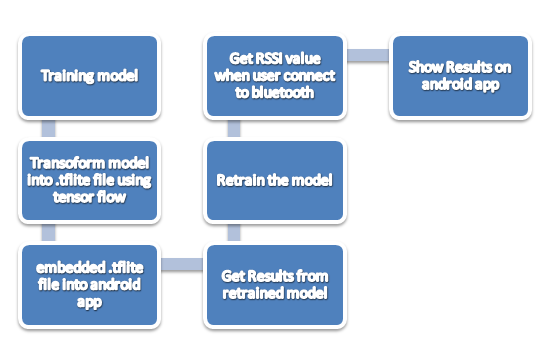
\includegraphics[scale=0.8]{./Figures/d1}
\caption{Steps to integrate the trained model}
\label{fig:17}
 		\end{figure}


\subsubsection{Functionality to turn ON bluetooth when users install the app}
When users install the app, he/she have to turn on the bluetooth. For this purpose, we add the functionality on android studio to turn on bluetooth.
Actually, Bluetooth is used to send or receive data between two devices. But, we used bluetooth only for scanning. Bluetooth scanned and get data of nearby devices such as Beacons and other bluetooth device. In this ways, we get the RSSI values and MAC Address of our beacons.
To implementation of this feature, we use bluetooth API which android provides. Android provides the class of Bluetooth Adapter. By using this class, we call the function of ACTION REQUEST ENABLE. This function used to enable the bluetooth for this app. Bluetooth is on and search nearby devices. To search nearby devices, we use the function ACTION REQUEST DISCOVERABLE.   It becomes discoverable for 120 seconds. We can extent it by using the function EXTRA-DISCOVERABLE-DURATION up to 1 hour (3600 seconds). 
After discover the nearby devices, we can get their RSSI values and MAC Address. The nearby devices which we discover, not only get the RSSI values and MAC Address of the beacons, but also get this data of other devices. Due to other devices our data become misclleneous.To get accurate data, we will remove this data and take it as missing value in data. 

\begin{figure}[h]
  		\centering
    		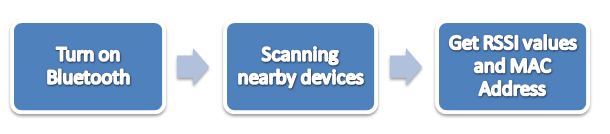
\includegraphics[scale=0.8]{./Figures/d2}
\caption{Steps to get RSSI values and MAC address}
\label{fig:18}
 		\end{figure}


\subsubsection{Make java classes to save RSSI values}
After scanning the bluetooth devices, we get the data of RSSI values and MAC Address of nearby devices. To save this data, we make java class named as Beacon.java. In this class, we take two strings variable that is as follows:
\begin{itemize}
\item RSSI  values 
\item MAC Address.
\end{itemize}
We can store these two variables in this class by using lists/ arrays. The different device has different RSSI values and MAC Address. Some other discoverable devices which are not our beacons also present. Their RSSI values and MAC Address also store in java class. But we want to remove this.
For this purpose, we make the function RemoveMisclleneousData(). In this function, we remove the misclleneous data from the list and take it as missing values.

\begin{figure}[h]
  		\centering
    		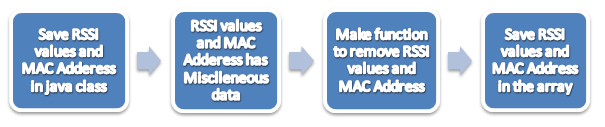
\includegraphics[scale=0.8]{./Figures/d3}
\caption{Steps to save RSSI values and MAC address in the array}
\label{fig:19}
 		\end{figure}


\subsubsection{Function to pass RSSI values to trained model}
After removing the misclleneous values from the java class, we pass list to the function. We made the function named passRSSIvalues(array[] RSSI , array MACaddr[]). In this function, we give the array of RSSI values and array of MAC Address as an input and take the Id of room as output in which the user is present. This function returns the Room Id. 
Actually, in our system, the RSSI values and MAC Addressed is labeled to the Room No. we also used the data labeling process for our system. The annotated data is present in our model file that is model.tflite.

\begin{figure}[h]
  		\centering
    		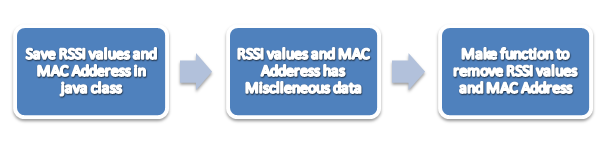
\includegraphics[scale=0.8]{./Figures/d4}
\caption{Steps to pass RSSI values to trained model}
\label{fig:20}
 		\end{figure}


\subsubsection{Show location of user}

After getting the Room Id, we give this room Id as an input to php MYSQL database server. We write a select query in php scripts which get data of Rooms, Room Member and their office hours.
 Using Admin App, we enter all the data of rooms. Now, in this time, we fetch the data from php MYSQL database server against this Room Id. The data is converted into JSON. We use JSON web services to fetch the data from database. Using these services, we get the data from php MYSQL and display this data on user’s screen. This data show the location of user on our User App.
\begin{figure}[h]
  		\centering
    		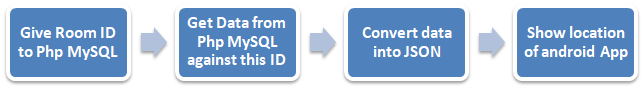
\includegraphics[scale=0.8]{./Figures/d5}
\caption{Steps to show location of user}
\label{fig:21}
 		\end{figure}

\subsubsection{Show all information of current room}
We have to show all the information of the room in which user is present. Actually, the admin app is used to enter the record in database but the user app is used to fetch the record from database. We use these tables to fetch the record from database that is:
\begin{itemize}
\item Room 
\item Room Members
\item Office Hours
\item Pictures
\item To show the information of the current room we follow some steps:
\item First of all, we create the activity.
\item In this activity we fetch the record of database
\item We fetch the pictures of the current room from Pictures table of database.
\item We fetch the audio from database of current room from the room table of database
\item We also show the description of that room. For this purpose, we fetch the room member name, area of expertise and designation from Room Member table.
\item We also fetch the office hour timings of room members of that current room from Office hour’s table to show the description of current room.
\end{itemize}


\subsubsection{Update location of the user}
As you all know, when we go to the new place, we want to visit that place. For this purpose, a person changes his position from one place to another. When person changes his position, we need to update the position of the person on android app. To implement this portion, we have to make the function named as UpdateUserLoc().  This function is used to update the location of the person on android App. When user changes his location, the location of the person also changes. We use delay time in this function. After 10 seconds, the location of the user will update.
\subsubsection{Show nearby location of the user}
The room ID which we get from the trained data, we give this room Id as an input to php MYSQL database server. We write a select query in php scripts to get the data of Rooms and nearby Rooms. 
Using Admin App, we enter all the data of rooms. In room table, Admin also enters the ID of nearby rooms such as room on left side, room on right side, room on front, room on back side of current room.  Now, in this time, we fetch the data of nearby rooms from php MYSQL database server against this Room Id. The data is converted into JSON. We use JSON web services to fetch the data from database. Using these services, we get the data from php MYSQL and display this data on user’s screen. This data shows the nearby location of user on our User Android App.
\subsubsection{Show all information of nearby rooms}
We have to show all the information of the nearby rooms. To show all the information of the nearby rooms we follow some steps:
\begin{itemize}
\item First of all, we create the activity for nearby rooms.
\item In this activity, we fetch the record of nearby rooms from database.
\item We fetch the pictures of the nearby rooms from Pictures table of database.
\item We fetch the audio from database of nearby rooms from the room table of database
\item We also show the description of nearby rooms. For this purpose, we fetch the room member name, area of expertise and designation from Room Member table.
\item We also fetch the office hour timings of room members of nearby rooms from Office hour’s table to show the description of nearby rooms.
\end{itemize}









